\documentclass{article}

% BASE TAKEN FROM ICCS315 SCRIBE NOTES

% --- SETUP STUFF ---
\usepackage[a4paper, margin=1in]{geometry}
\usepackage{enumitem}
\usepackage{booktabs}

\usepackage{url}
\usepackage[unicode]{hyperref}

\setcounter{secnumdepth}{2}

% --- MATH STUFF ---
\usepackage{amsthm, amsmath, amssymb}
\usepackage{mathtools,xspace}
\usepackage{nicefrac}

\usepackage{bbm}
\usepackage{dsfont}
\usepackage{cancel}

\usepackage{blkarray}
\newcommand{\matindex}[1]{\mbox{\scriptsize#1}} % Matrix index

% --- FONT STUFF ---
% Has to be under math stuff for some reason :/
\usepackage{newpxtext, newpxmath}
\usepackage[T1]{fontenc}

% --- DIAGRAM STUFF ---
\usepackage{tikz,pgfplots,xcolor,graphicx}
\usepackage{graphicx}
\usepackage{colortbl}
\usepackage{caption}
\usepackage{subcaption}

\usepackage[breakable,skins]{tcolorbox}
\usepackage{framed}
\usepackage{float}

\pgfplotsset{compat=1.18}

% --- THEOREM STUFF ---
\newtheorem{theorem}{Theorem}[section]
\newtheorem{proposition}[theorem]{Proposition}
\newtheorem{lemma}[theorem]{Lemma}
\newtheorem{corollary}[theorem]{Corollary}

\theoremstyle{definition}
\newtheorem{definition}[theorem]{Definition}
\newtheorem{example}[theorem]{Example}

\theoremstyle{remark}
\newtheorem{remark}[theorem]{Remark}
\newtheorem{claim}[theorem]{Claim}
\newtheorem{fact}[theorem]{Fact}

\usepackage{algorithm}
\usepackage[indLines=true]{algpseudocodex}
\usepackage{algorithmicx}
\algnewcommand\algorithmicinput{\textbf{Input:}}
\algnewcommand\Input{\item[\algorithmicinput]}
\algrenewcommand\algorithmicoutput{\textbf{Output:}}
\algrenewcommand\Output{\item[\algorithmicoutput]}
\algrenewcommand\algorithmicrequire{\textbf{Require:}}
\algrenewcommand\Require{\item[\algorithmicrequire]}

\renewcommand{\Pr}[1]{\mathbf{Pr}\left[#1\right]}
\newcommand{\CPr}[2]{\mathbf{Pr}\left[#1\ |\ #2\right]}
\newcommand{\Ex}[1]{\mathbf{E}\left[#1\right]}
\newcommand{\ExSub}[2]{\mathbf{E}_#2\left[#1\right]}
\newcommand{\CEx}[2]{\mathbf{E}\left[#1\ |\ #2\right]}

\newcommand{\Exp}[1]{\text{Exp}\left(#1\right)}
\newcommand{\Pois}[1]{\text{Poisson}\left(#1\right)}
\newcommand{\DGamma}[2]{\text{Gamma}\left(#1, #2\right)}
\DeclareMathOperator{\diam}{diam}

% === NOTES PORTION ===
% \begin{document}
%
% \frontmatter
% \thispagestyle{empty}

\begin{center}
\vspace{5cm}

\Huge{Graph Theory}

\vspace{5em}
\begin{center}
  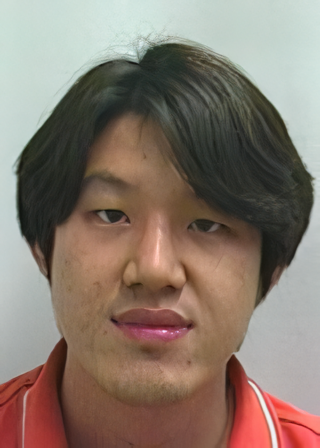
\includegraphics[height=0.5\textheight]{figures/chad.png}
\end{center}
\vspace{5em}

\Large Student's Notes for {T2/2023-2024}

\Large Written by {Nawat Ngerncham}

\Large Last updated: \today
\end{center}

%
% \setcounter{tocdepth}{1}
% \tableofcontents
%
% \mainmatter

% === HOMEWORK PORTION ===
\title{\Huge{In-class Problem 1}
	\\
\Large\scshape{{Graph Theory and Combinatorics}}}
\author{{Nawat Ngerncham}}
\date{\today}

\begin{document}

\maketitle

\section*{Notations}

\begin{figure}[ht]
  \begin{center}
    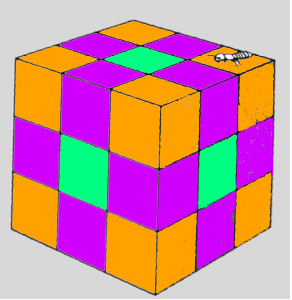
\includegraphics[width=0.3\textwidth]{figures/cube}
  \end{center}
  \caption{Outer layer}\label{fig:cube}
\end{figure}

Let us define the following notations for the blocks on the outer layer based on
Figure \ref{fig:cube}. Note that the only block in the center---the
center---will just be called the center.

\begin{itemize}
  \item The \textit{corners} will refer to the {\color{orange}orange} part of 
    the cube
  \item The \textit{mid} will refer to the {\color{teal}green} part of the cube
  \item The \textit{surround} will refer to the {\color{purple}purple} part of
    the cube
\end{itemize}

\section*{Solution}

\begin{claim}
  There is no Hamiltonian Path from any of the outer 26 blocks that ends up at the center.
\end{claim}

\begin{proof}
  We can represent each block as a vertex in a graph. Then, for each vertex, we
  can find its degree by counting the number of blocks it has around it.
  \begin{itemize}
    \item There is 1 center, each connected to 6 mids
    \item There are 6 mids, each connected to 4 surrounds and 1 center
    \item There are 12 surrounds, each connected to 2 mids and to 2 corners
    \item There are 8 corners, each connected to 3 surround
  \end{itemize}

  Since the adjacency/connection implies that a 2-way traversal is possible, we
  will start our traversal from the center block and show that it is impossible
  to visit every cube without repeating. Notice the following pattern. Namely,
  we can see that once we leave the center block, we will always end up at a mid
  block. Then, we are forced to visit a surround block since we cannot go back
  into the center. After that, we have the choice of visiting a corner or
  another mid block. Hence, we can create the following graph in Figure
  \ref{fig:graph} (similar to a Markov Chain) to represent the different types
  of blocks the termite will end up at.

  \begin{figure}[ht]
    \centering
    \tikzset{every picture/.style={line width=0.75pt}} %set default line width to 0.75pt        

    \begin{tikzpicture}[x=0.75pt,y=0.75pt,yscale=-1,xscale=1]
    %uncomment if require: \path (0,369); %set diagram left start at 0, and has height of 369

    %Shape: Circle [id:dp11052413892947599] 
    \draw  [fill={rgb, 255:red, 255; green, 255; blue, 255 }  ,fill opacity=1 ] (41,100.5) .. controls (41,77.58) and (59.58,59) .. (82.5,59) .. controls (105.42,59) and (124,77.58) .. (124,100.5) .. controls (124,123.42) and (105.42,142) .. (82.5,142) .. controls (59.58,142) and (41,123.42) .. (41,100.5) -- cycle ;
    %Shape: Circle [id:dp7640336273930843] 
    \draw  [fill={rgb, 255:red, 255; green, 255; blue, 255 }  ,fill opacity=1 ] (225,98.5) .. controls (225,75.58) and (243.58,57) .. (266.5,57) .. controls (289.42,57) and (308,75.58) .. (308,98.5) .. controls (308,121.42) and (289.42,140) .. (266.5,140) .. controls (243.58,140) and (225,121.42) .. (225,98.5) -- cycle ;
    %Shape: Circle [id:dp7316521615959588] 
    \draw  [fill={rgb, 255:red, 255; green, 255; blue, 255 }  ,fill opacity=1 ] (453,97.5) .. controls (453,74.58) and (471.58,56) .. (494.5,56) .. controls (517.42,56) and (536,74.58) .. (536,97.5) .. controls (536,120.42) and (517.42,139) .. (494.5,139) .. controls (471.58,139) and (453,120.42) .. (453,97.5) -- cycle ;
    %Shape: Circle [id:dp6227688105474427] 
    \draw  [fill={rgb, 255:red, 255; green, 255; blue, 255 }  ,fill opacity=1 ] (461,305.5) .. controls (461,282.58) and (479.58,264) .. (502.5,264) .. controls (525.42,264) and (544,282.58) .. (544,305.5) .. controls (544,328.42) and (525.42,347) .. (502.5,347) .. controls (479.58,347) and (461,328.42) .. (461,305.5) -- cycle ;
    %Straight Lines [id:da784133928479497] 
    \draw    (124,100.5) -- (223,98.54) ;
    \draw [shift={(225,98.5)}, rotate = 178.87] [color={rgb, 255:red, 0; green, 0; blue, 0 }  ][line width=0.75]    (10.93,-3.29) .. controls (6.95,-1.4) and (3.31,-0.3) .. (0,0) .. controls (3.31,0.3) and (6.95,1.4) .. (10.93,3.29)   ;
    %Curve Lines [id:da21195468919891436] 
    \draw    (308,98.5) .. controls (342.3,83.31) and (422.7,83.97) .. (451.31,96.71) ;
    \draw [shift={(453,97.5)}, rotate = 206.57] [color={rgb, 255:red, 0; green, 0; blue, 0 }  ][line width=0.75]    (10.93,-3.29) .. controls (6.95,-1.4) and (3.31,-0.3) .. (0,0) .. controls (3.31,0.3) and (6.95,1.4) .. (10.93,3.29)   ;
    %Curve Lines [id:da8200298461285411] 
    \draw    (453,97.5) .. controls (409.44,124.73) and (353.14,121.08) .. (309.32,99.17) ;
    \draw [shift={(308,98.5)}, rotate = 27.08] [color={rgb, 255:red, 0; green, 0; blue, 0 }  ][line width=0.75]    (10.93,-3.29) .. controls (6.95,-1.4) and (3.31,-0.3) .. (0,0) .. controls (3.31,0.3) and (6.95,1.4) .. (10.93,3.29)   ;
    %Curve Lines [id:da22618846468106057] 
    \draw    (494.5,139) .. controls (529.29,168.4) and (517.5,234.3) .. (503.37,262.33) ;
    \draw [shift={(502.5,264)}, rotate = 298.24] [color={rgb, 255:red, 0; green, 0; blue, 0 }  ][line width=0.75]    (10.93,-3.29) .. controls (6.95,-1.4) and (3.31,-0.3) .. (0,0) .. controls (3.31,0.3) and (6.95,1.4) .. (10.93,3.29)   ;
    %Curve Lines [id:da04435189848385512] 
    \draw    (492.94,140.77) .. controls (459.51,179.76) and (476.4,237.41) .. (502.5,264) ;
    \draw [shift={(494.5,139)}, rotate = 132.31] [color={rgb, 255:red, 0; green, 0; blue, 0 }  ][line width=0.75]    (10.93,-3.29) .. controls (6.95,-1.4) and (3.31,-0.3) .. (0,0) .. controls (3.31,0.3) and (6.95,1.4) .. (10.93,3.29)   ;

    % Text Node
    \draw (58,83) node [anchor=north west][inner sep=0.75pt]   [align=left] {\begin{minipage}[lt]{33.34pt}\setlength\topsep{0pt}
    \begin{center}
    Center\\(1)
    \end{center}

    \end{minipage}};
    % Text Node
    \draw (253,81) node [anchor=north west][inner sep=0.75pt]   [align=left] {\begin{minipage}[lt]{19.16pt}\setlength\topsep{0pt}
    \begin{center}
    Mid\\(6)
    \end{center}

    \end{minipage}};
    % Text Node
    \draw (462,80) node [anchor=north west][inner sep=0.75pt]   [align=left] {\begin{minipage}[lt]{44.68pt}\setlength\topsep{0pt}
    \begin{center}
    Surround\\(12)
    \end{center}

    \end{minipage}};
    % Text Node
    \draw (476,286) node [anchor=north west][inner sep=0.75pt]   [align=left] {\begin{minipage}[lt]{33.9pt}\setlength\topsep{0pt}
    \begin{center}
    Corner\\(8)
    \end{center}
    \end{minipage}};
    \end{tikzpicture}
    \caption{Traversal pattern between different types of blocks}
    \label{fig:graph}
  \end{figure}

  In order to visit every block, we have to leave the center, visit different 
  mids totaling exactly 6 times, visit different surrounds totaling exactly 
  12 times, and visit different corners totaling exactly 8 times in some
  order. However, notice that we can only traverse from mid to corner by first
  visiting surround. Since we cannot repeat vertices, it follows that it is
  impossible to visit every mid and corner blocks without repeated visits to some
  surround blocks because
  \[ \text{\# mids} + \text{\# corners} = 6 + 8 > 12 = \text{\# surrounds} \]
  Thus, there is no Hamiltonian Path from any block on the outer layer that that
  ends at the center block. Therefore, it is impossible for a termite to start
  from an outer center (mid), visit every block, and end at the center block. 
\end{proof}


% in case of needing citations
% \bibliographystyle{plainurl}
% \bibliography{refs}

\end{document}
